\documentclass[tikz,border=10pt]{standalone}
\usepackage{pgfplots}
\usepgfplotslibrary{fillbetween}
\pgfplotsset{every axis plot post/.append style =
  {samples=80, smooth, thick, black, mark=none} }
\begin{document}
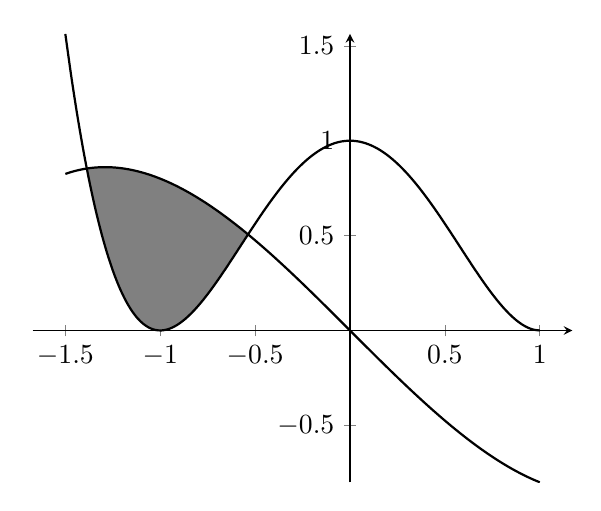
\begin{tikzpicture}
  \begin{axis}[axis lines = center, axis equal,
      domain = -1.5:1]
    \addplot[name path=cubic]   {x^3/5 - x};
    \addplot[name path=quartic] {(x^2-1)^2};
    \addplot fill between[of=cubic and quartic, split,
      every segment/.style = {transparent},
      every segment no 1/.style = {gray,opaque}];
  \end{axis}
\end{tikzpicture}
\end{document}
